% % % % % % % % % % % % % % % % % % % % % % % % % % % % % % % % % % % % % % % %
% IEEE Style - Double columns, 11pt font, letterpaper
\documentclass[journal, twocolumn, final,11pt,letterpaper]{IEEEtran}	

% Include Latex Packages
\usepackage{etex}	% This package enables the use of many packages

% % Page styles
\usepackage{setspace}	% line spacing package
\doublespacing			% use double spacing
%\linespread{1.6}		% Use linespread to fine tune line spacing, not recommended


% % Figures
\usepackage{float}		% improves interface for floating objects
\usepackage{subfig}		% enables subfloat
\usepackage{graphicx}	% more image type support
\usepackage{circuitikz}
\usepackage{epstopdf}	% automatically convert included eps files to pdf
\usepackage{tikz}
%\usepackage{listings}
\usepackage{color}
\definecolor{dkgreen}{rgb}{0,0.6,0}
\definecolor{gray}{rgb}{0.5,0.5,0.5}
\definecolor{mauve}{rgb}{0.58,0,0.82}

\lstset{frame=tb,
	language=Verilog,
	aboveskip=3mm,
	belowskip=3mm,
	showstringspaces=false,
	columns=flexible,
	basicstyle={\small\ttfamily},
	numbers=none,
	numberstyle=\tiny\color{gray},
	keywordstyle=\color{blue},
	commentstyle=\color{dkgreen},
	stringstyle=\color{mauve},
	breaklines=true,
	breakatwhitespace=true,
	tabsize=3
}
\usetikzlibrary{matrix,calc}
\usetikzlibrary{shapes}

\newcommand*{\circled}[2][red]{
	\tikz[baseline=(char.base)]{
		\node[shape=ellipse,inner sep=1pt,
		draw=#1,
		] (char) {#2};}
}

%isolated term
%#1 - Optional. Space between node and grouping line. Default=0
%#2 - node
%#3 - filling color
\newcommand{\implicantsol}[3][0]{
	\draw[rounded corners=3pt, fill=#3, opacity=0.3] ($(#2.north west)+(135:#1)$) rectangle ($(#2.south east)+(-45:#1)$);
}


%internal group
%#1 - Optional. Space between node and grouping line. Default=0
%#2 - top left node
%#3 - bottom right node
%#4 - filling color
\newcommand{\implicant}[4][0]{
	\draw[rounded corners=3pt, fill=#4, opacity=0.3] ($(#2.north west)+(135:#1)$) rectangle ($(#3.south east)+(-45:#1)$);
}

%group lateral borders
%#1 - Optional. Space between node and grouping line. Default=0
%#2 - top left node
%#3 - bottom right node
%#4 - filling color
\newcommand{\implicantcostats}[4][0]{
	\draw[rounded corners=3pt, fill=#4, opacity=0.3] ($(rf.east |- #2.north)+(90:#1)$)-| ($(#2.east)+(0:#1)$) |- ($(rf.east |- #3.south)+(-90:#1)$);
	\draw[rounded corners=3pt, fill=#4, opacity=0.3] ($(cf.west |- #2.north)+(90:#1)$) -| ($(#3.west)+(180:#1)$) |- ($(cf.west |- #3.south)+(-90:#1)$);
}

%group top-bottom borders
%#1 - Optional. Space between node and grouping line. Default=0
%#2 - top left node
%#3 - bottom right node
%#4 - filling color
\newcommand{\implicantdaltbaix}[4][0]{
	\draw[rounded corners=3pt, fill=#4, opacity=0.3] ($(cf.south -| #2.west)+(180:#1)$) |- ($(#2.south)+(-90:#1)$) -| ($(cf.south -| #3.east)+(0:#1)$);
	\draw[rounded corners=3pt, fill=#4, opacity=0.3] ($(rf.north -| #2.west)+(180:#1)$) |- ($(#3.north)+(90:#1)$) -| ($(rf.north -| #3.east)+(0:#1)$);
}

%group corners
%#1 - Optional. Space between node and grouping line. Default=0
%#2 - filling color
\newcommand{\implicantcantons}[2][0]{
	\draw[rounded corners=3pt, opacity=.3] ($(rf.east |- 0.south)+(-90:#1)$) -| ($(0.east |- cf.south)+(0:#1)$);
	\draw[rounded corners=3pt, opacity=.3] ($(rf.east |- 8.north)+(90:#1)$) -| ($(8.east |- rf.north)+(0:#1)$);
	\draw[rounded corners=3pt, opacity=.3] ($(cf.west |- 2.south)+(-90:#1)$) -| ($(2.west |- cf.south)+(180:#1)$);
	\draw[rounded corners=3pt, opacity=.3] ($(cf.west |- 10.north)+(90:#1)$) -| ($(10.west |- rf.north)+(180:#1)$);
	\fill[rounded corners=3pt, fill=#2, opacity=.3] ($(rf.east |- 0.south)+(-90:#1)$) -|  ($(0.east |- cf.south)+(0:#1)$) [sharp corners] ($(rf.east |- 0.south)+(-90:#1)$) |-  ($(0.east |- cf.south)+(0:#1)$) ;
	\fill[rounded corners=3pt, fill=#2, opacity=.3] ($(rf.east |- 8.north)+(90:#1)$) -| ($(8.east |- rf.north)+(0:#1)$) [sharp corners] ($(rf.east |- 8.north)+(90:#1)$) |- ($(8.east |- rf.north)+(0:#1)$) ;
	\fill[rounded corners=3pt, fill=#2, opacity=.3] ($(cf.west |- 2.south)+(-90:#1)$) -| ($(2.west |- cf.south)+(180:#1)$) [sharp corners]($(cf.west |- 2.south)+(-90:#1)$) |- ($(2.west |- cf.south)+(180:#1)$) ;
	\fill[rounded corners=3pt, fill=#2, opacity=.3] ($(cf.west |- 10.north)+(90:#1)$) -| ($(10.west |- rf.north)+(180:#1)$) [sharp corners] ($(cf.west |- 10.north)+(90:#1)$) |- ($(10.west |- rf.north)+(180:#1)$) ;
}

%Empty Karnaugh map 4x4
\newenvironment{Karnaugh}%
{
	\begin{tikzpicture}[baseline=(current bounding box.north),scale=0.8]
	\draw (0,0) grid (4,4);
	\draw (0,4) -- node [pos=0.9,above right,anchor=south west] {C1C0} node [pos=0.9,below left,anchor=north east] {EQ} ++(135:1);
	%
	\matrix (mapa) [matrix of nodes,
	column sep={0.8cm,between origins},
	row sep={0.8cm,between origins},
	every node/.style={minimum size=0.3mm},
	anchor=8.center,
	ampersand replacement=\&] at (0.5,0.5)
	{
		\& |(c00)| 00         \& |(c01)| 01         \& |(c11)| 11         \& |(c10)| 10         \& |(cf)| \phantom{00} \\
		|(r00)| 00             \& |(0)|  \phantom{0} \& |(1)|  \phantom{0} \& |(3)|  \phantom{0} \& |(2)|  \phantom{0} \&                     \\
		|(r01)| 01             \& |(4)|  \phantom{0} \& |(5)|  \phantom{0} \& |(7)|  \phantom{0} \& |(6)|  \phantom{0} \&                     \\
		|(r11)| 11             \& |(12)| \phantom{0} \& |(13)| \phantom{0} \& |(15)| \phantom{0} \& |(14)| \phantom{0} \&                     \\
		|(r10)| 10             \& |(8)|  \phantom{0} \& |(9)|  \phantom{0} \& |(11)| \phantom{0} \& |(10)| \phantom{0} \&                     \\
		|(rf) | \phantom{00}   \&                    \&                    \&                    \&                    \&                     \\
	};
}%
{
	\end{tikzpicture}
}

%Empty Karnaugh map 2x4
\newenvironment{Karnaughvuit}%
{
	\begin{tikzpicture}[baseline=(current bounding box.north),scale=0.8]
	\draw (0,0) grid (4,2);
	\draw (0,2) -- node [pos=0.7,above right,anchor=south west] {LA/LB} node [pos=0.6,below left,anchor=north east] {S} ++(120:1);
	%
	\matrix (mapa) [matrix of nodes,
	column sep={0.8cm,between origins},
	row sep={0.8cm,between origins},
	every node/.style={minimum size=0.3mm},
	anchor=4.center,
	ampersand replacement=\&] at (0.5,0.5)
	{
		\& |(c00)| 00         \& |(c01)| 01         \& |(c11)| 11         \& |(c10)| 10         \& |(cf)| \phantom{00} \\
		|(r00)| 0             \& |(0)|  \phantom{0} \& |(1)|  \phantom{0} \& |(3)|  \phantom{0} \& |(2)|  \phantom{0} \&                     \\
		|(r01)| 1             \& |(4)|  \phantom{0} \& |(5)|  \phantom{0} \& |(7)|  \phantom{0} \& |(6)|  \phantom{0} \&                     \\
		|(rf) | \phantom{00}  \&                    \&                    \&                    \&                    \&                     \\
	};
}%
{
	\end{tikzpicture}
}

%Empty Karnaugh map 2x2
\newenvironment{Karnaughquatre}%
{
	\begin{tikzpicture}[baseline=(current bounding box.north),scale=0.8]
	\draw (0,0) grid (2,2);
	\draw (0,2) -- node [pos=0.7,above right,anchor=south west] {b} node [pos=0.7,below left,anchor=north east] {a} ++(135:1);
	%
	\matrix (mapa) [matrix of nodes,
	column sep={0.8cm,between origins},
	row sep={0.8cm,between origins},
	every node/.style={minimum size=0.3mm},
	anchor=2.center,
	ampersand replacement=\&] at (0.5,0.5)
	{
		\& |(c00)| 0          \& |(c01)| 1  \\
		|(r00)| 0 \& |(0)|  \phantom{0} \& |(1)|  \phantom{0} \\
		|(r01)| 1 \& |(2)|  \phantom{0} \& |(3)|  \phantom{0} \\
	};
}%
{
	\end{tikzpicture}
}

%Defines 8 or 16 values (0,1,X)
\newcommand{\contingut}[1]{%
	\foreach \x [count=\xi from 0]  in {#1}
	\path (\xi) node {\x};
}

%Places 1 in listed positions
\newcommand{\minterms}[1]{%
	\foreach \x in {#1}
	\path (\x) node {1};
}

%Places 0 in listed positions
\newcommand{\maxterms}[1]{%
	\foreach \x in {#1}
	\path (\x) node {0};
}

%Places X in listed positions
\newcommand{\indeterminats}[1]{%
	\foreach \x in {#1}
	\path (\x) node {X};
}



% % Maths
\usepackage[cmex10]{amsmath}	% Maths
\usepackage{amsfonts,amssymb} 	% maths symbols

% % Tables
\usepackage{booktabs}  % professional-looking tables
\usepackage{multicol} %used for getting multicolumn without page-break
\usepackage{multirow}	% multi-row tables
\usepackage{array}		% define column format of a table

% % Others
\usepackage{caption}	%Customising captions in floating environments
%\usepackage{abstract}
\usepackage{cite}		% cite multiple
\usepackage{fixltx2e}	%added by pilawa, preventing figure* to get ahead of regular figures.
\usepackage{url}		% url display

% %
\hyphenation{op-tical net-works semi-conduc-tor}	% correct bad hyphenation here
\providecommand{\e}[1]{\ensuremath{\times 10^{#1}}}		% use use \e{2} for scientific number expression


% % Optional packages that might be useful
%\usepackage{epsf}		% eps fix
%\usepackage{verbatim}	% verbatim text are not interpreted by the compiler 
%\numberwithin{equation}{section}	% number equation according to section
%\usepackage{xfrac}		% slanted fraction
%\usepackage{pgfplots}	% plot graph
%\usepackage{tikz,pgfplots} % plot graph
%\usepackage{endnotes}	% endnotes


% Title of Document
\title{ECE385 Experiment \#4
	}
\author{
\IEEEauthorblockN{Eric Meyers, Ryan Helsdingen}\\
\IEEEauthorblockA{Section ABG; TAs: Ben Delay, Shuo Liu \\
February 17th, 2016 \\
emeyer7, helsdin2}}
% % % % % % % % % % % % % % % % % % % % % % % % % % % % % % % % % % % % % % % 
\begin{document}
	
%SECTION : Formatting and Title
\maketitle
\singlespacing

%SECTION 1 - Introduction - Eric
\section{Introduction}
\IEEEPARstart{T}{he} purpose of this lab was to get a brief introduction to System Verilog and Quartus by creating and analyzing a total of 4 designs. The first is an 8 bit serial logic processor that was created during last lab (Lab 3) using TTL chips on a breadboard. The next three being different configurations of 16-bit adders: A carry-ripple adder, a carry-lookahead adder, and a carry-select adder. The team then analyzed the performance of these three adders by selecting different metrics to compare as well as analyzed the performance of the serial logic processor compared to the design used in Lab 3.

%SECTION 2 - Schematic of Logic Processor -Eric  
\section{Schematic of Logic Processor}
Please refer to Figure \ref{fig:schematic-processor} in "Section XI: Figures" to view the Schematic of the 8-bit Logic Processor designed in the Pre-Lab of this Experiment.

%SECTION 3 - Design Simulations - Eric
\section{Design Simulations of Logic Processor}
Please refer to Figure \ref{fig:processor-output-rtl-simulator} in "Section XI: Figures" to view the Annotated RTL Simulation Output of the 8-bit Logic Processor designed in the Pre-Lab of this Experiment.

%SECTION 4 - Written Description - Ryan 
\section{Written Description of Adder Circuit}
The three adders used in this lab were the carry-ripple adder (CRA), carry-select adder (CSA), and the carry-lookahead adder (CLA).  All three designs manipulated in some way or another the full adder.  As you can see in the full adder block diagram (Fig. \ref{fig:full-adder-block-schematic}) and full adder truth table (Table \ref{FAtruth}, the full adder has two logic inputs, a carry-in bit input, and two outputs including a sum bit and a carry-out bit.  The full adders function is to add all three input bits and send any access bits to the carry-out bit.  In other words, the sum and carry-out bit form a two bit sum of the three inputs with the sum being the less significant bit.  \\
   
\begin{center}
	\begin{tabular}{lll|ll}
		A & B &$C_{in}$& $C_{out}$& S \\ \hline
		0 & 0 & 0      & 0 & 0\\
		0 & 0 & 1      & 0 & 1\\
		0 & 1 & 0      & 0 & 1\\
		0 & 1 & 1      & 1 & 0\\
		1 & 0 & 0      & 0 & 1\\
		1 & 0 & 1      & 1 & 0\\
		1 & 1 & 0      & 1 & 0\\
		1 & 1 & 1      & 1 & 1\\		
	\end{tabular}
	\label{FAtruth}
\end{center}

The first adder designed, the CRA,  was the most straightfoward approach to an N-bit binary adder.  It consisted of a chain of full adders connected by their carry bits. The first adder would have a carry-in bit of logic 0.  It would take in the least significant bit of both register A and B (A[0] and B[0]) and add the two, outputting the least significant sum bit (S[0]) and a carry-out bit that would link to the carry-in bit of the next full adder.  This chain would continue for all 16 bits.  While this design is simple, long computation time is its biggest issue.  Later full adders must wait for a signal in their carry-in bits in order to function correctly.  One adder alone, has several gates the signal must go through before a carry-out signal is generated.  \\

The next adder designed was the CLA.  It brought in a method that would reduce the wait time that the CRA suffered from.  This method took the CRA design and replaced the carry-out bit of the full adder with both a generating (G) bit and a propagating (P) bit.  Each full adder would then take in input bits A and B and do a little educated guesswork with them.  The G bit checked for two high bits, guaranteeing that the carry-in of the next full adder would be high.  It followed G=A$\cdot$B.  The P bit checked for only one of the two to be high.  It followed P=A+B, and would serve as a potential for a logic 1 to be sent to the next full adder.  The last possible result of A and B inputs, that is, both are low, would output a low P and G bit giving no chance for the next carry-in bit to be logic 1.  The carry-in bit of the next adder thus held a logical expression of $C_{i+1}=G_i+(P_i\cdot C_i)$.  This new method cuts down the computation time compared to the CRA by predetermining the next carry-in bit if inputs bits A and B share the same signal.  Unfortunately the CLA uses more logic gates at the cost of area and power consumption.  \\

The final adder designed was the CSA.  This design was the least-straightforward of the three designs.  Each bit required two full-adders, a 2-to-1 mux, an AND gate, and an OR gate.  Both full-adders would take in the same A and B input bits.  One full-adder would simulate a logic 0 for the carry-in bit and send its sum bit to the 0 input on the 2-to-1 mux.  Likewise, the other full-adder would simulate a logic 1 for the carry-in bit and send its sum output bit the 1 input of the 2-to-1 mux.  The output of the mux is the sum bit for that one-bit CSA and would be selected through the value of the carry-in bit for the one-bit CSA. The carry-out of the full-adder with the logic 1 carry-in gets AND'd with the carry-in of the one-bit CSA and that result gets OR'd with the carry-out of the full-adder with the logic 0 carry-in.  The result is the carry-out bit of the one-bit CSA which gets sent to the carry-in bit of the next one-bit CSA.  This design cuts down on computation time by precomputing both possibilities of carry-in bits.  However, this design uses the most logic gates which increases both power consumption and area.  \\


%SECTION 5 - Purpose of Modules - Ryan
\section{Purpose of Modules}
For the CRA, only full-adders were used to add each bit.  The need for modules was not necessary for this design, so it manipulated the flat approach.  However, for the CLA and CSA, 4-bit modules were created to optimize speed.  The number of gates per bit of adding was quite higher for these two designs.  A flat approach would have been impractical especially for 16 bit addition or greater.  Instead, a hierarchical approach was used.  Both the CLA and CSA used 4-bit modules.  \\

The CLA 4-bit module contained four copies of the one-bit CLA. The carry-in bit of the least significant bit acted as the carry-in bit of the module and the carry-out bit of the most significant bit acted as the carry-out bit of the module.  The module took in four input bits for A and B sending them to their respective one-bit CLA inputs and outputted four sum bits, one from each one-bit CLA.  Connecting the modules was a simple wire connecting the carry-out of one module to the carry-in of the next high significant 4-bit module.  The 16-bit CLA had therefore 4x4-bit modules connected.\\

The same process was used with the CSA except that each module contained (4) 1-bit CSA.  Also the need for guessing the carry-in bit on the least significant 4-bit module was unnecessary since it was guaranteed to be logic 0, so a 4-bit full-adder replaced it. \\

%SECTION 6 - State Machine - Eric
\section{State Machine}
The State Machine for the Serial Bit Logic Processor Control Unit is shown in Figure  \ref{fig:serial-processor-state-machine} in "Section XI: Figures" of this document.  \\

The State Machine is broken down into a total of ten states labeled A through J, with A being the initial/halt state and J being the final state. The intermediary states are the shifting states (eight in total meaning that the shift register shifts eight times before coming to a halt).
	
%SECTION 7 - Schematic/Block Diagrams -Ryan 
\section{Schematic Block Diagrams}
All block diagrams are shown in Figures \ref{fig:full-adder-block-schematic} to \ref{fig:one-bit-csa-block-schematic} found in "Section XI: Figures" of this document.  Block diagrams show in order the CRA basic full adder block digram, then the CLA block diagrams, and finally the CSA block diagrams.  For the CLA and CSA block digrams, first the 4x4-bit system block digram is shown, then the block diagram for a 4-bit module is shown, and lastly the one-bit block diagram is shown.    


%SECTION 8 - Design Analysis - Eric
\section{Design Analysis Comparison}
The following table displays the values the team received upon analyzing the metrics requested in the pre-lab.
\begin{center}
	\begin{tabular}{l|lll}
		Metric & Ripple & Lookahead & Select \\ \hline
		Memory(BRAM) & 0 & 0 & 0 \\
		Frequency (MHz) & 62.81 & 64.526 & 61.55\\
		Power (mW) & 156.65 & 156.39 & 156.30\\
	\end{tabular}
\end{center}

The following figure 

\begin{figure} [H]
	\centering
	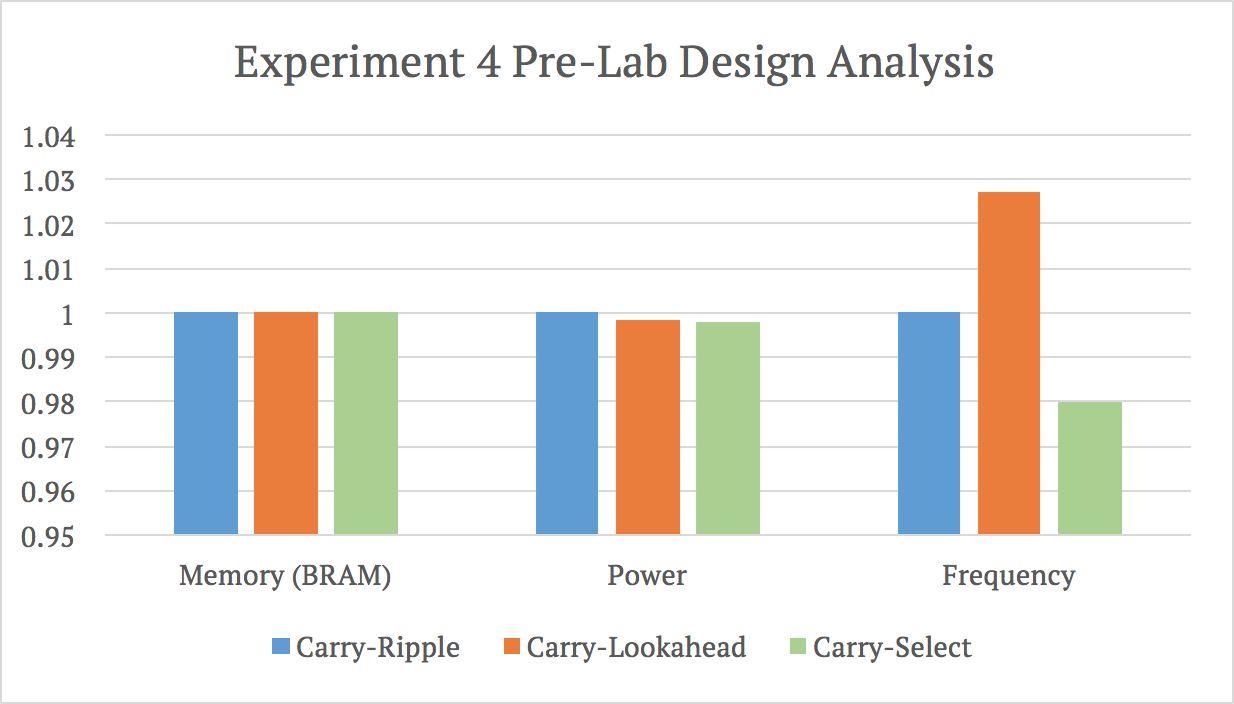
\includegraphics[scale=0.35]{pre-lab-design-analysis.png}
	\caption{Area, Power, Frequency Comparison\label{fig:pre-lab-design-analysis}}
\end{figure}


%SECTION 9 - Post Lab - Eric
\section{Post-Lab}
1) Compare the usage of LUT, Memory, and Flip-Flop of your bit-serial logic processor
exercise in the IQT with your TTL design in Lab 3. Make an educated guess of the usage of
these resources for TTL assuming the processor is extended to 8-bit. Which design is better, and
why? \\

\textit{Answer:} The System Verilog design used in Lab 4 clearly dominates the total usage of Logic Elements in Lab 3 almost by a factor of three. This is because the system used in Lab4 is very efficient and optimizes/reduces the amount of Logic Elements used as neccessary. However, this was not done in Lab 3 efficiently. If the team attempted to do Lab 3 again, a lower LE count would have been achieved but no where near the efficiency of using Quartus.
\begin{table} [H]
	\centering
	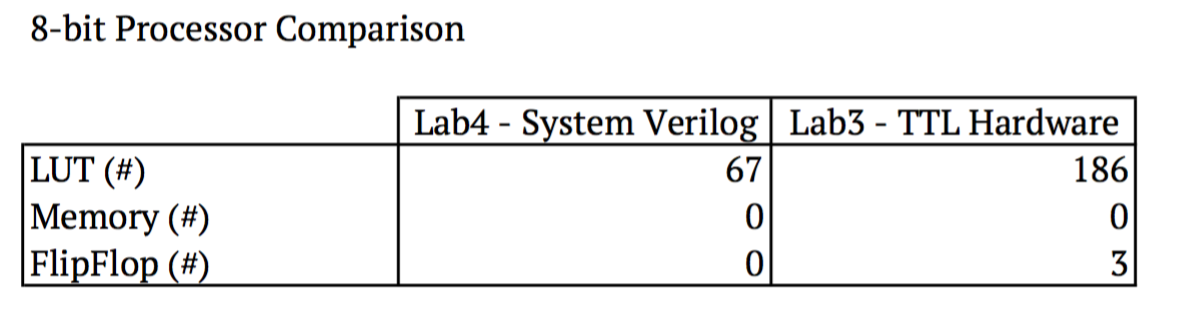
\includegraphics[scale=0.35]{processor-comparison.png}
	\caption{Processor Area Comparison\label{tab:processor-comparison}}
\end{table}

2) For the adders, refer to the Design Resources and Statistics in IQT.30-32 and complete
the following design statistics table for each adder. This is more comprehensive than the above
design analysis and is required for every SystemVerilog circuit.\\

These numbers are shown below in Table \ref{tab:lab4-statistics} .

\begin{table} [H]
	\centering
	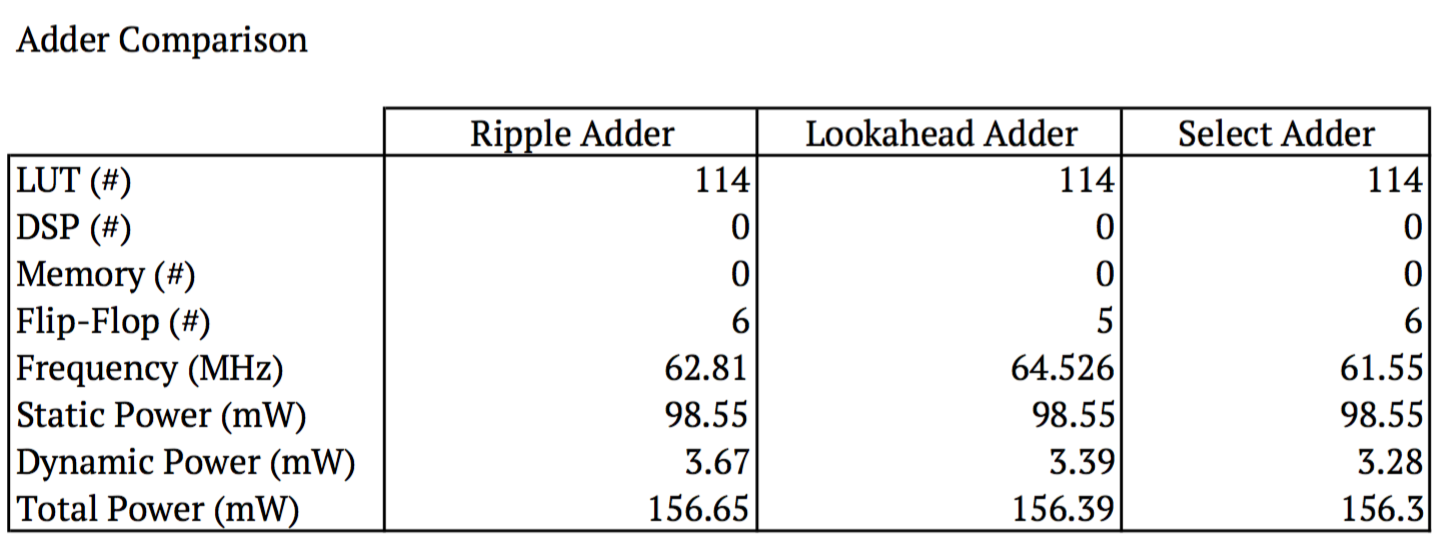
\includegraphics[scale=0.35]{lab4-statistics.png}
	\caption{Processor Area Comparison\label{tab:lab4-statistics}}
\end{table}

Observe the data plot and provide explanation to the data, i.e., does each resource
breakdown comparison from the plot makes sense? Are they complying with the theoretical
design expectations, e.g., the maximum operating frequency of the carry-lookahead adder is
higher than the carry-ripple adder? Which design consumes more power than the other as you
expected, why?\\

\textit{Answer:} The frequency of the Lookahead Adder was, indeed, faster than that of the Ripple Adder or the Select Adder. This makes sense because, although the Lookahead Adder consumes more area through logic elements (must connect each adder together with some logic so that the next adder can see the carry bits), it is faster which is shown in the frequency analysis.\\

The only result that was somewhat surprising to the group was that the Select Adder was slower than the Ripple Adder. The team was not sure why this was the case because the Select Adder should \textit{usually} be slower than the Ripple Adder however, not in this case.

%SECTION 10 - Conclusion - Eric
\section{Conclusion}
Overall, the team successfully demonstrated all three different adder configurations (Carry-Ripple, Carry-Lookahead, and Carry-Select) during the demo period for full credit. These adders were analyzed in the previous sections and it is evident that the Lookahead Adder was the fastest out of all three, and the Select Adder consumed the least amount of power out of all three.\\

The serial bit logic processor created in the pre-lab outperformed the bit logic processor constructed in lab 3 in several manners. For one, the total number of logic elements on the System Verilog Processor was $\approx$ 60 while the TTL Lab 3 total logic elements was exceeding $\approx$  180. This is almost a factor of three reduction because of Quartus optimization techniques and improvements to the circuit.\\ 

Overall, the team gained plenty of insight to the benefits of using System Verilog vs. using TTL chips on breadboards. The complexity decreased significantly and breaking sequential and combinational logic into modules through System Verilog proves to be a very effective. 


\clearpage
\onecolumn
%SECTION 11: Figures
\section{Figures}

\begin{figure} [htbp]
	\centering
	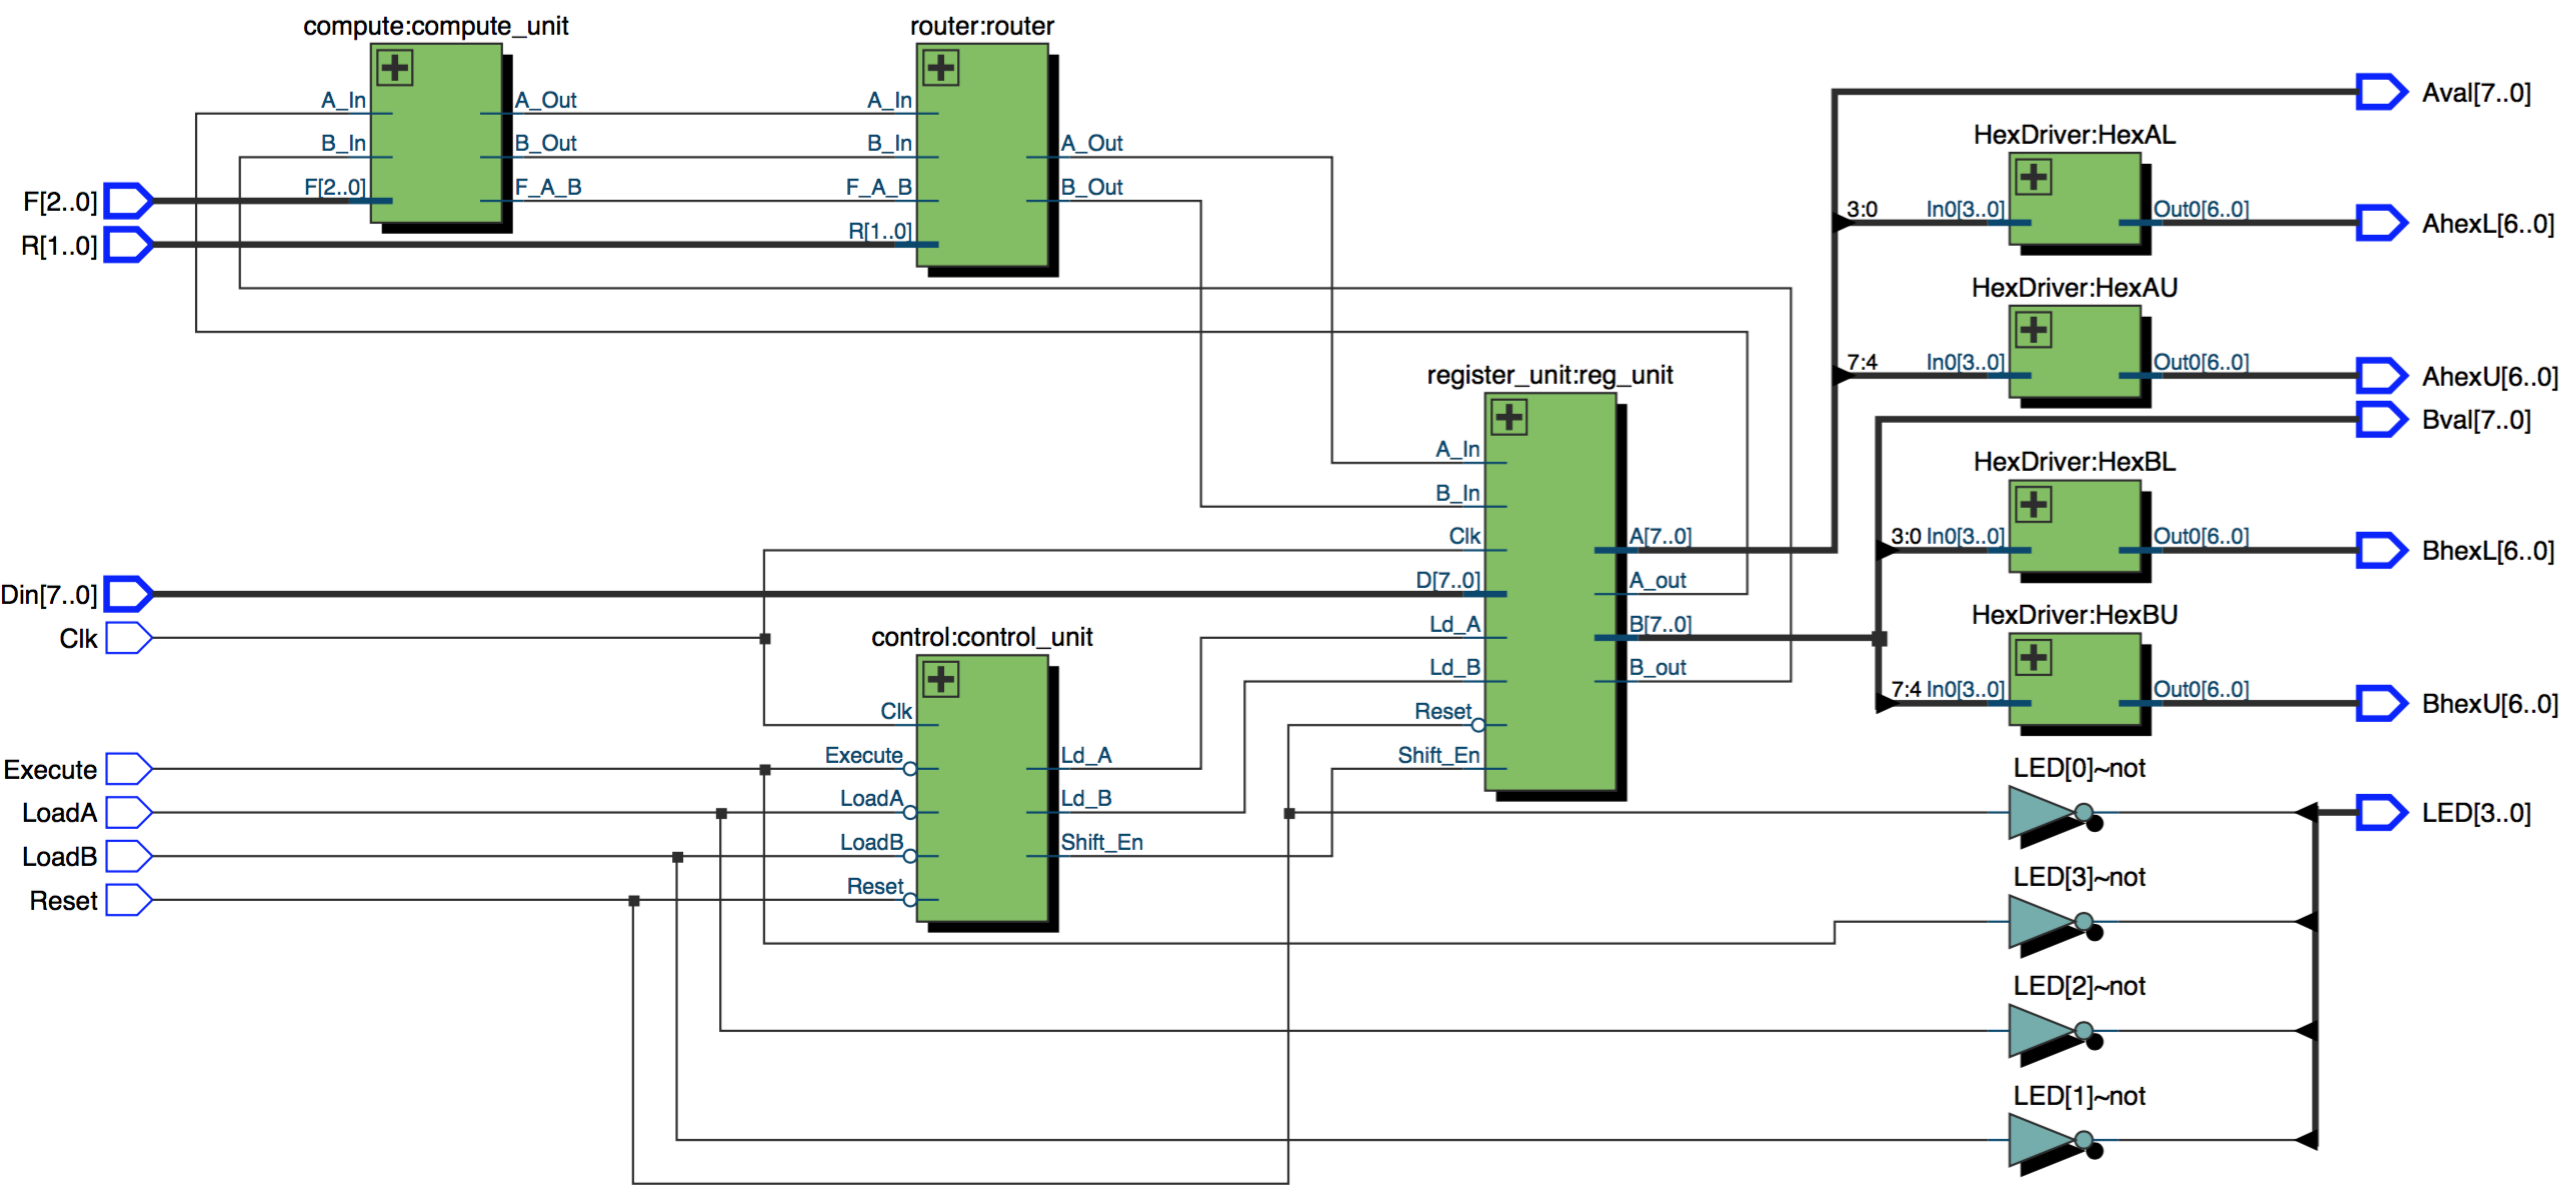
\includegraphics[scale=0.35]{Schematic-Processor.png}
	\caption{Serial Logic Processor Schematic\label{fig:schematic-processor}}
\end{figure}

\begin{figure} [htbp]
	\centering
	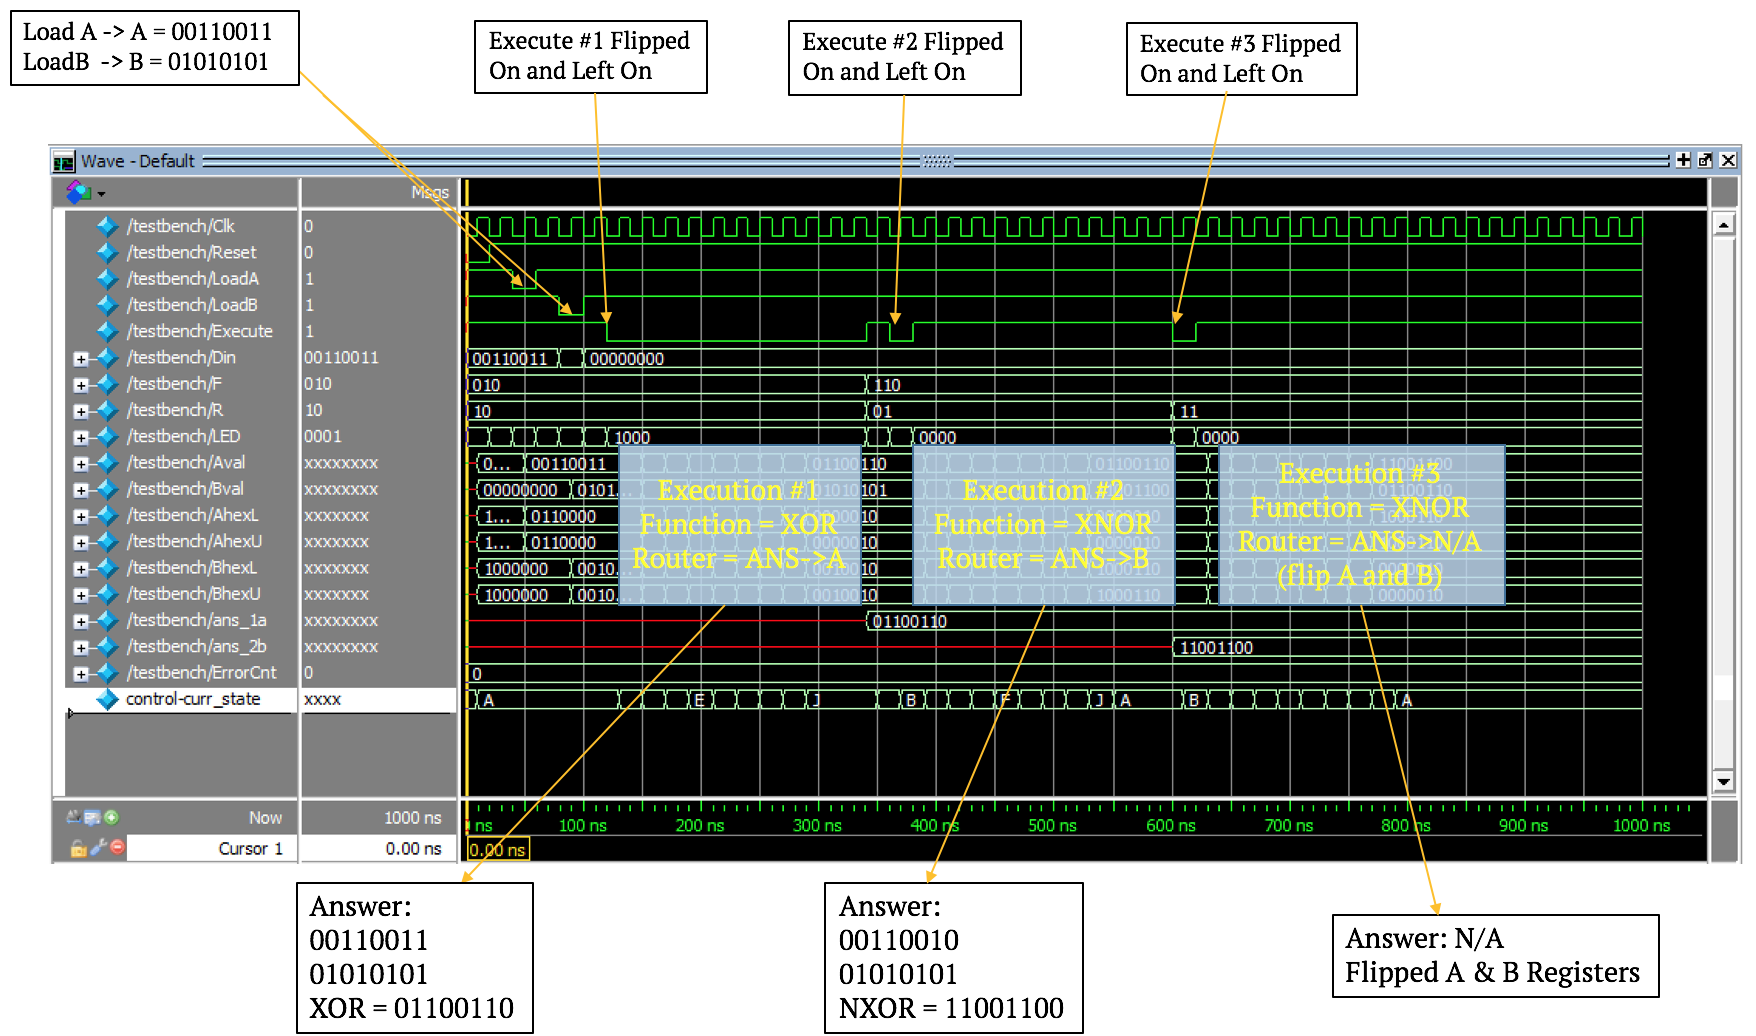
\includegraphics[scale=0.55]{processor-output-rtl-simulator.png}
	\caption{Serial Logic Processor RTL Simulation Output\label{fig:processor-output-rtl-simulator}}
\end{figure}

\begin{figure} [htbp]
	\centering
	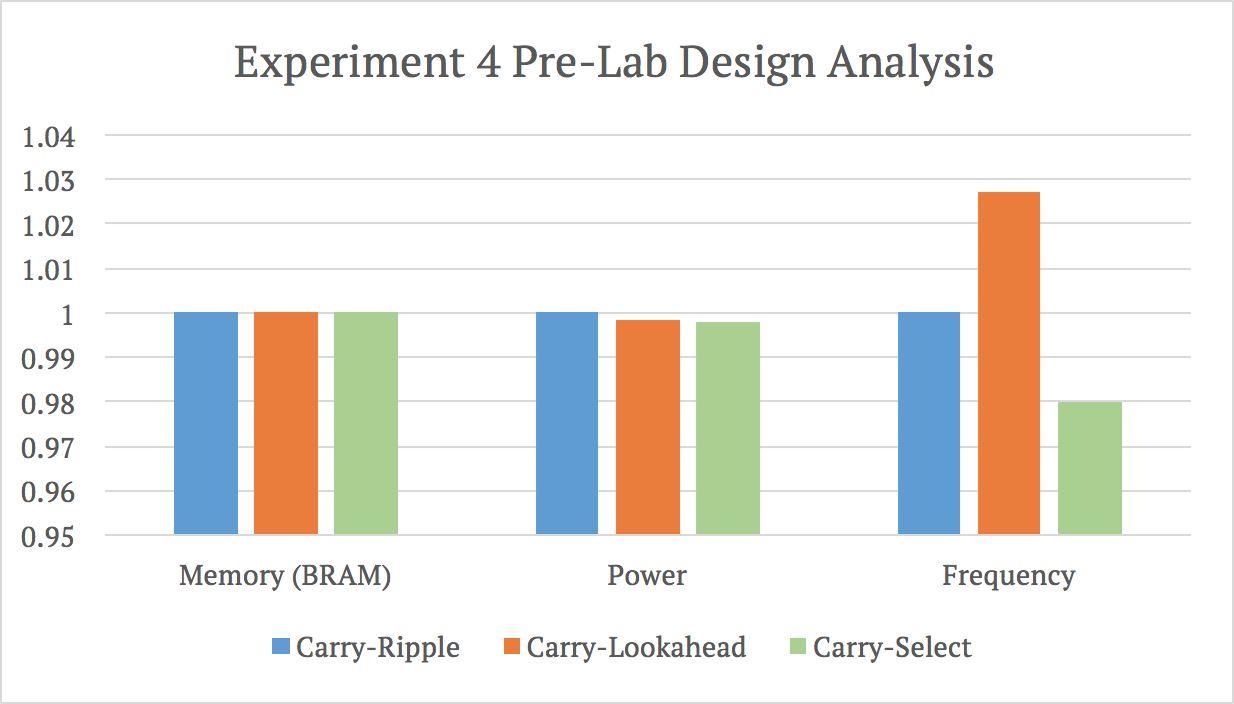
\includegraphics[scale=0.55]{pre-lab-design-analysis.png}
	\caption{Pre-Lab Adder Design Analysis (Area, Power, Frequency)\label{fig:pre-lab-design-analysis}}
\end{figure}

\begin{figure} [htbp]
	\centering
	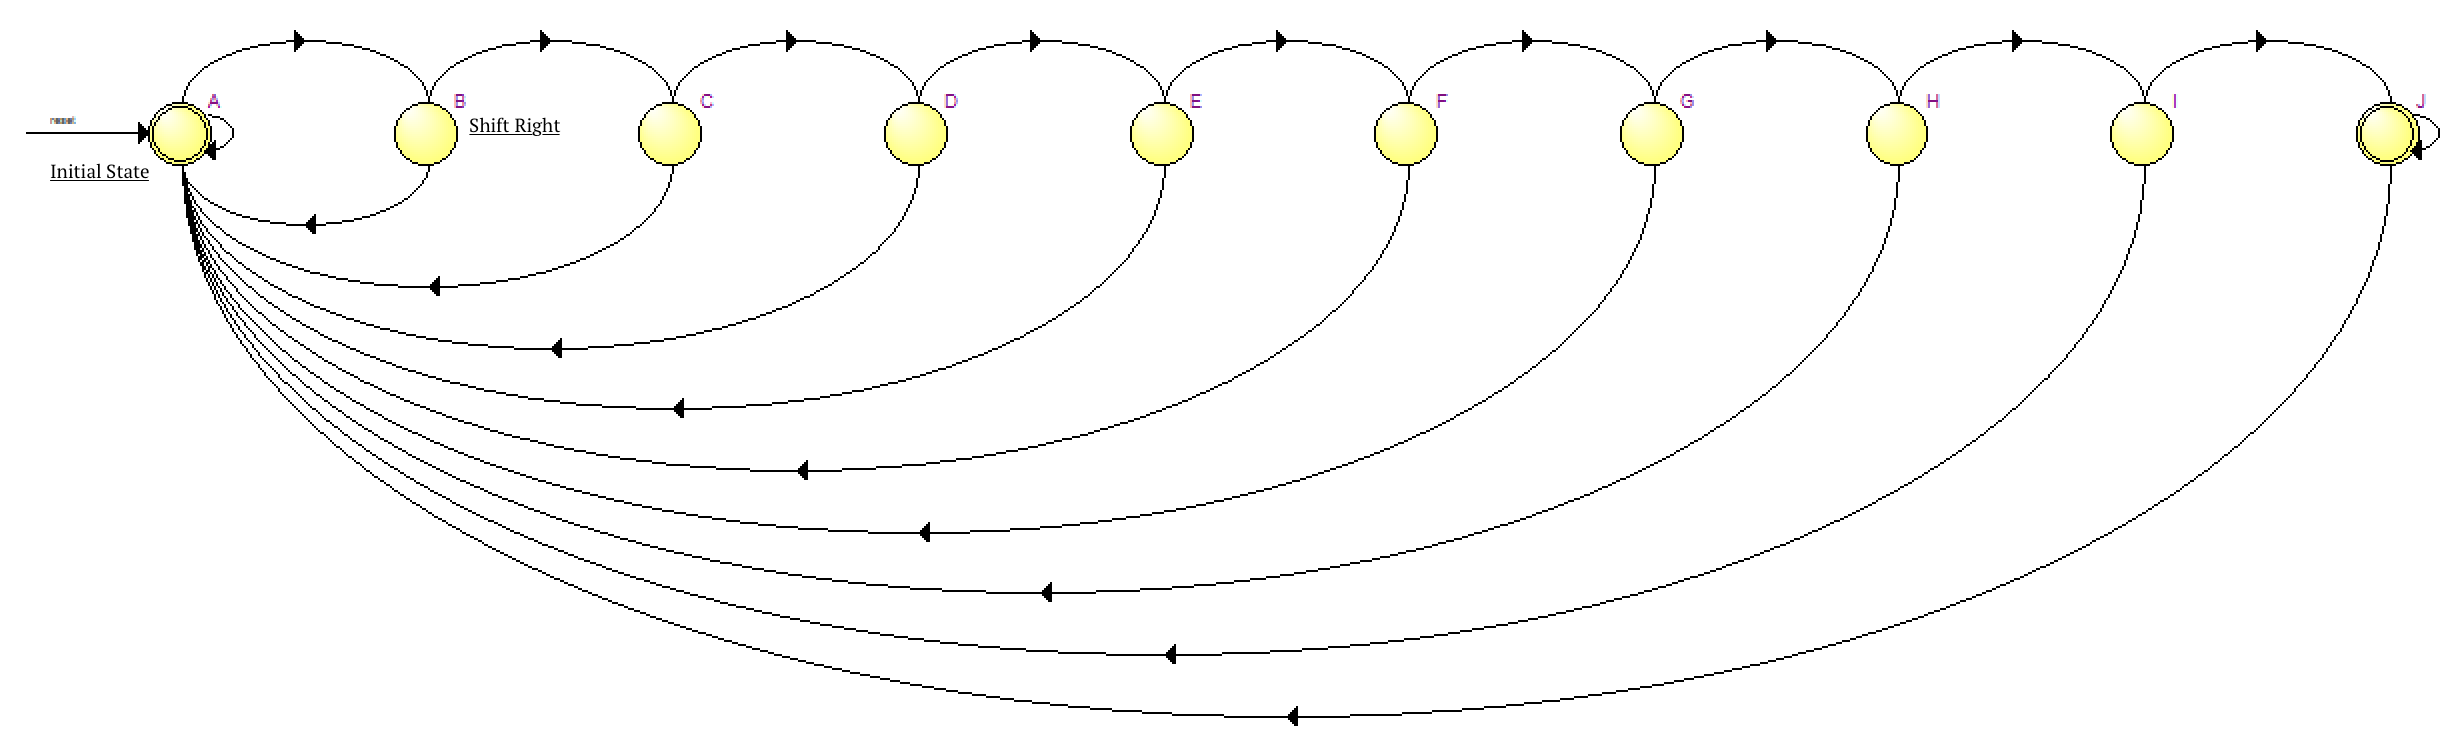
\includegraphics[scale=0.4]{state-machine-processor.png}
	\caption{State Machine for Serial Bit Logic Processor \label{fig:serial-processor-state-machine}}
\end{figure}

\begin{figure} [htbp]
	\centering
	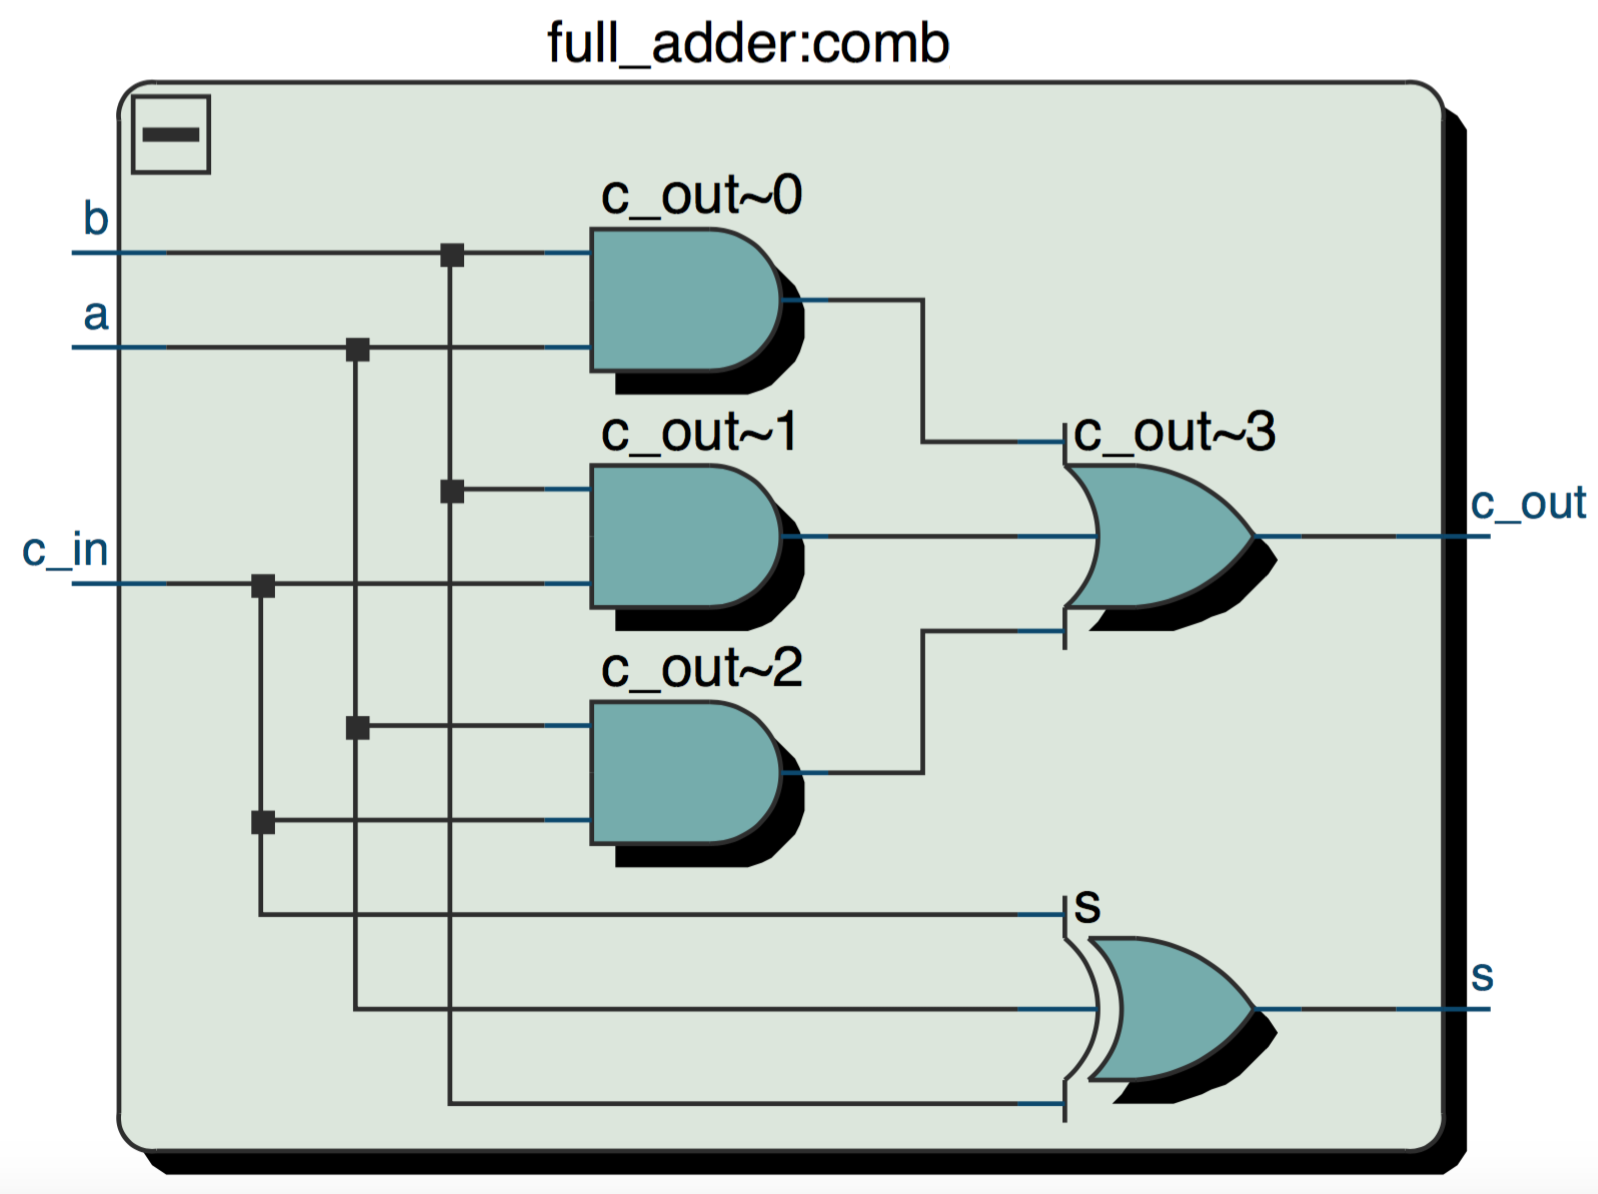
\includegraphics[scale=0.4]{full-adder-block-schematic.png}
	\caption{Full-Adder Block Schematic\label{fig:full-adder-block-schematic}}
\end{figure}

\begin{figure} [htbp]
	\centering
	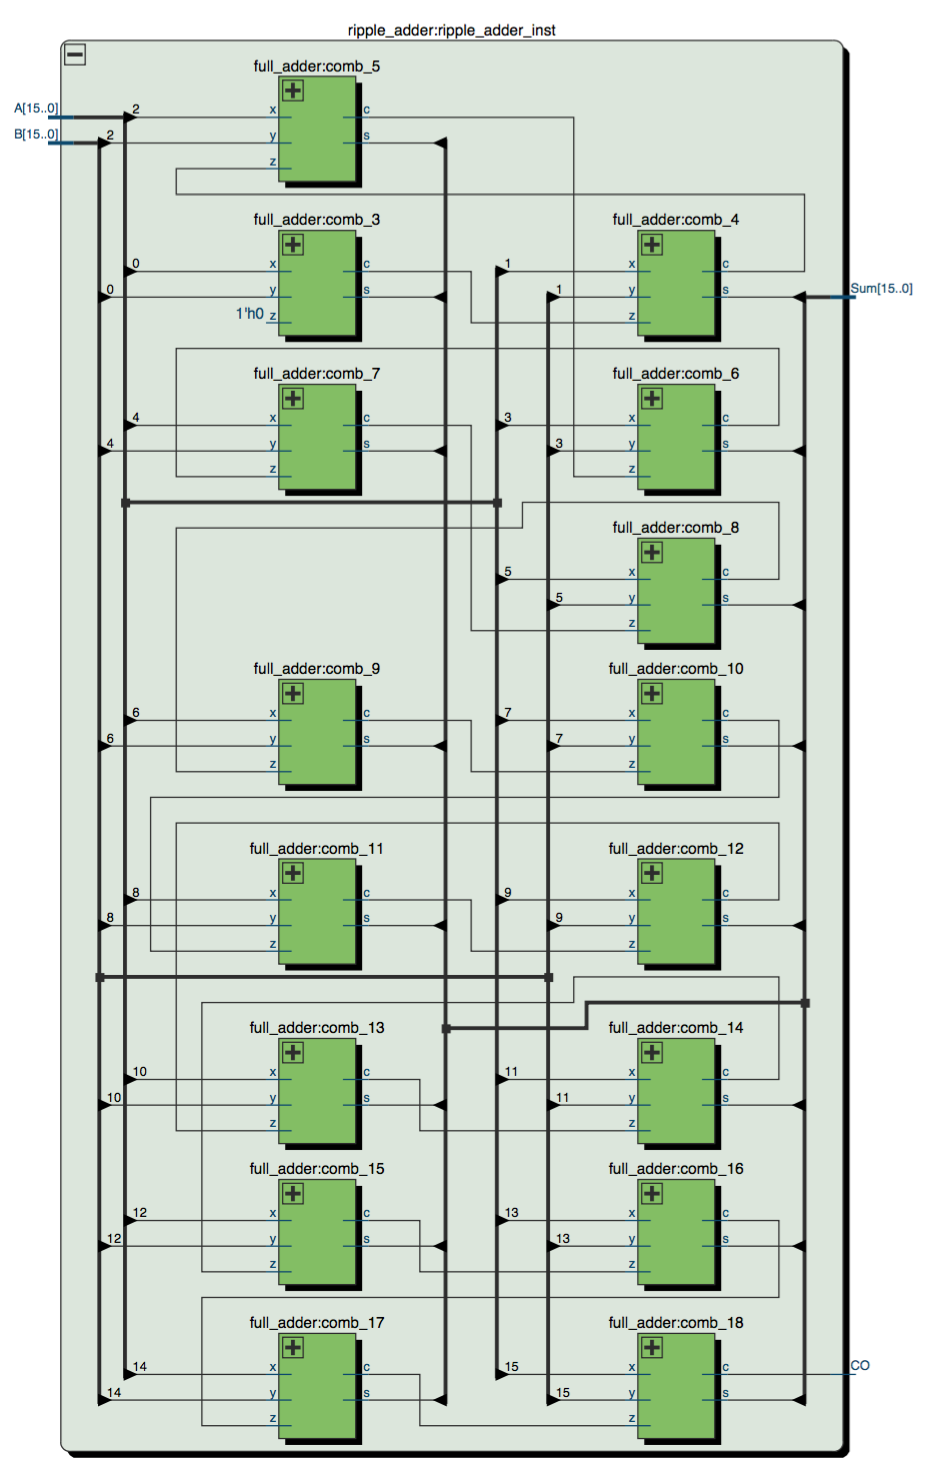
\includegraphics[scale=0.4]{carry-ripple-block-schematic.png}
	\caption{Carry Ripple Block Schematic\label{fig:carry-ripple-block-schematic}}
\end{figure}

\begin{figure} [htbp]
	\centering
	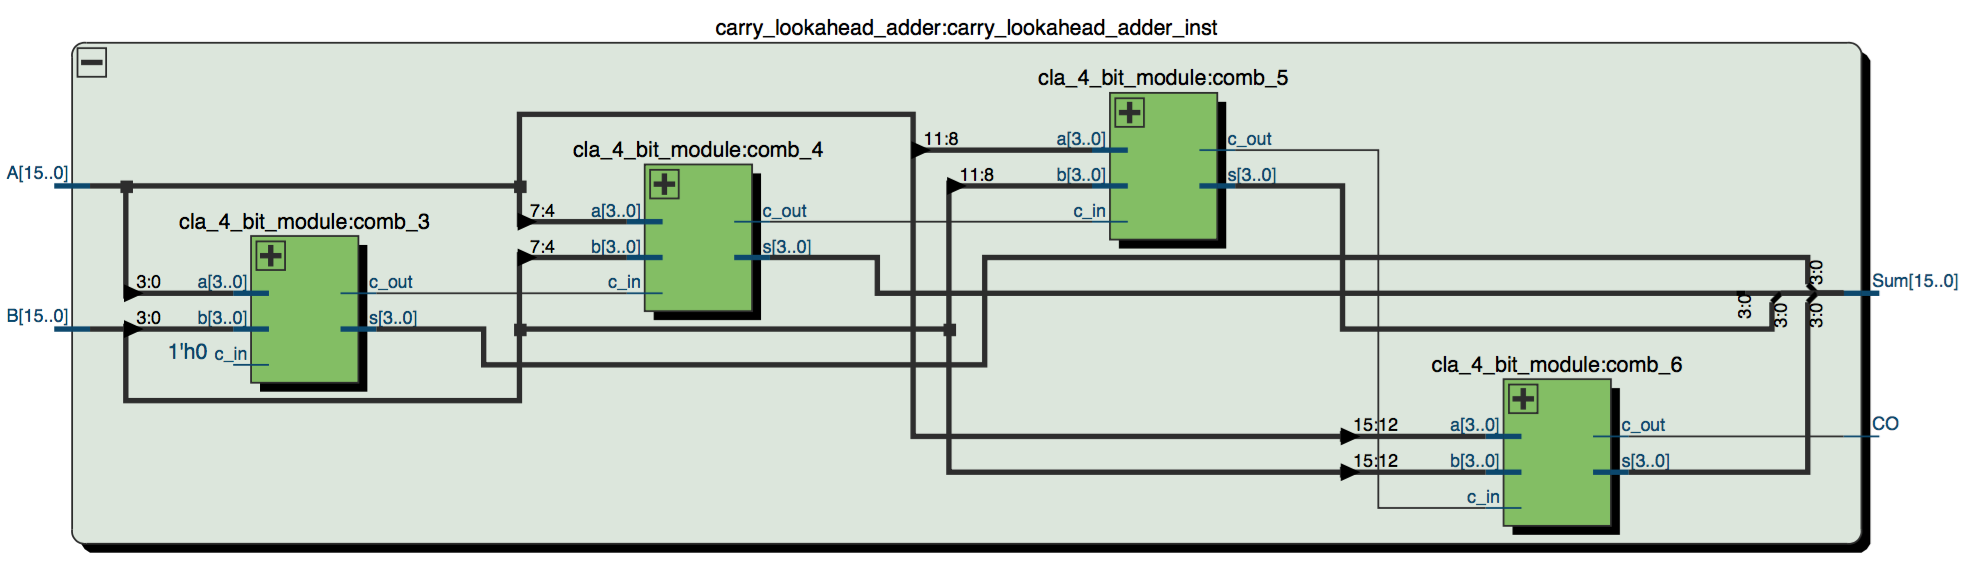
\includegraphics[scale=0.4]{carry-lookahead-block-schematic.png}
	\caption{Carry Lookahead (CLA) Block Schematic\label{fig:carry-lookahead-block-schematic}}
\end{figure}

\begin{figure} [htbp]
	\centering
	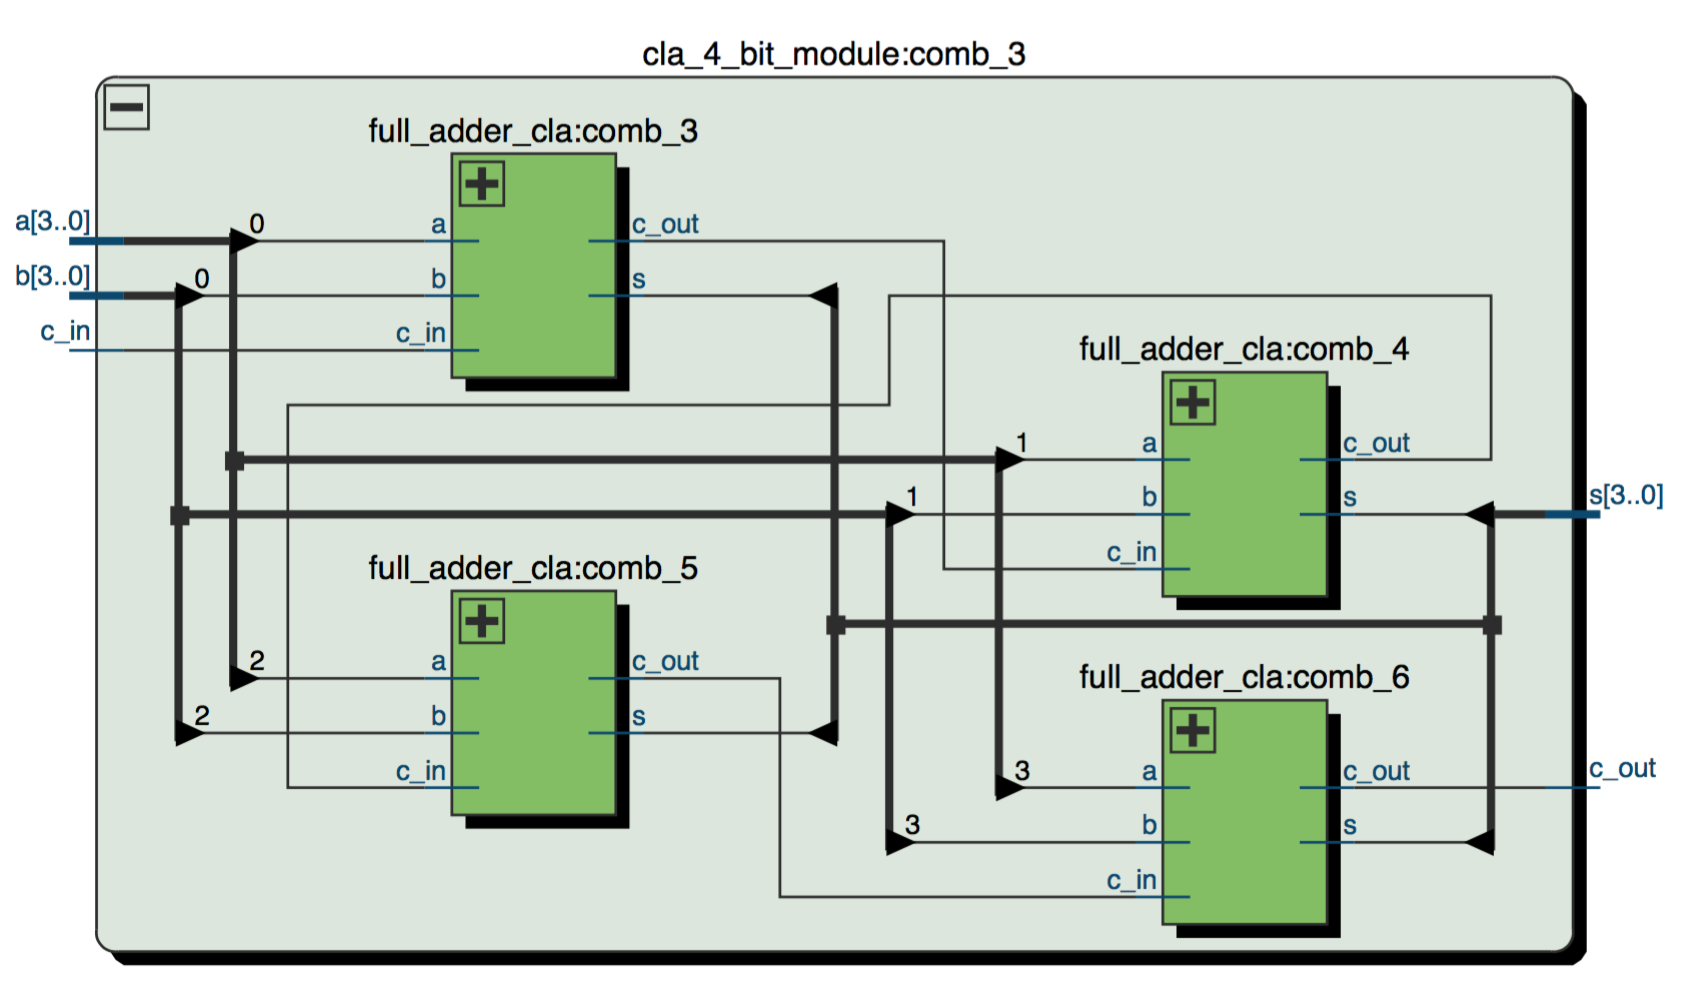
\includegraphics[scale=0.4]{four-bit-cla-block-schematic.png}
	\caption{Four-Bit CLA Block Schematic\label{fig:four-bit-cla-block-schematic}}
\end{figure}

\begin{figure} [htbp]
	\centering
	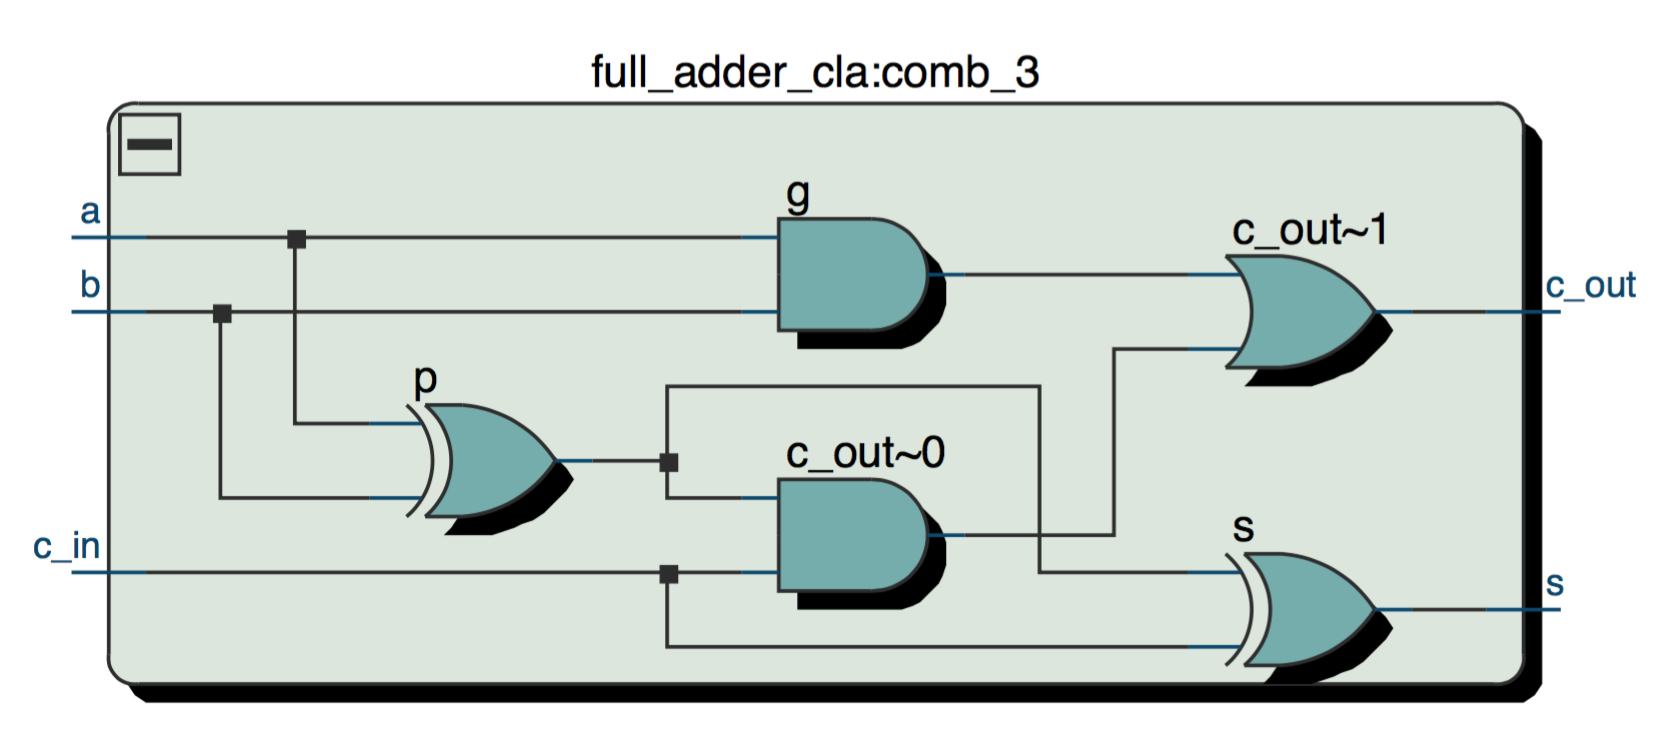
\includegraphics[scale=0.4]{one-bit-cla-block-schematic.png}
	\caption{One-Bit CLA Block Schematic\label{fig:one-bit-cla-block-schematic}}
\end{figure}


\begin{figure} [htbp]
	\centering
	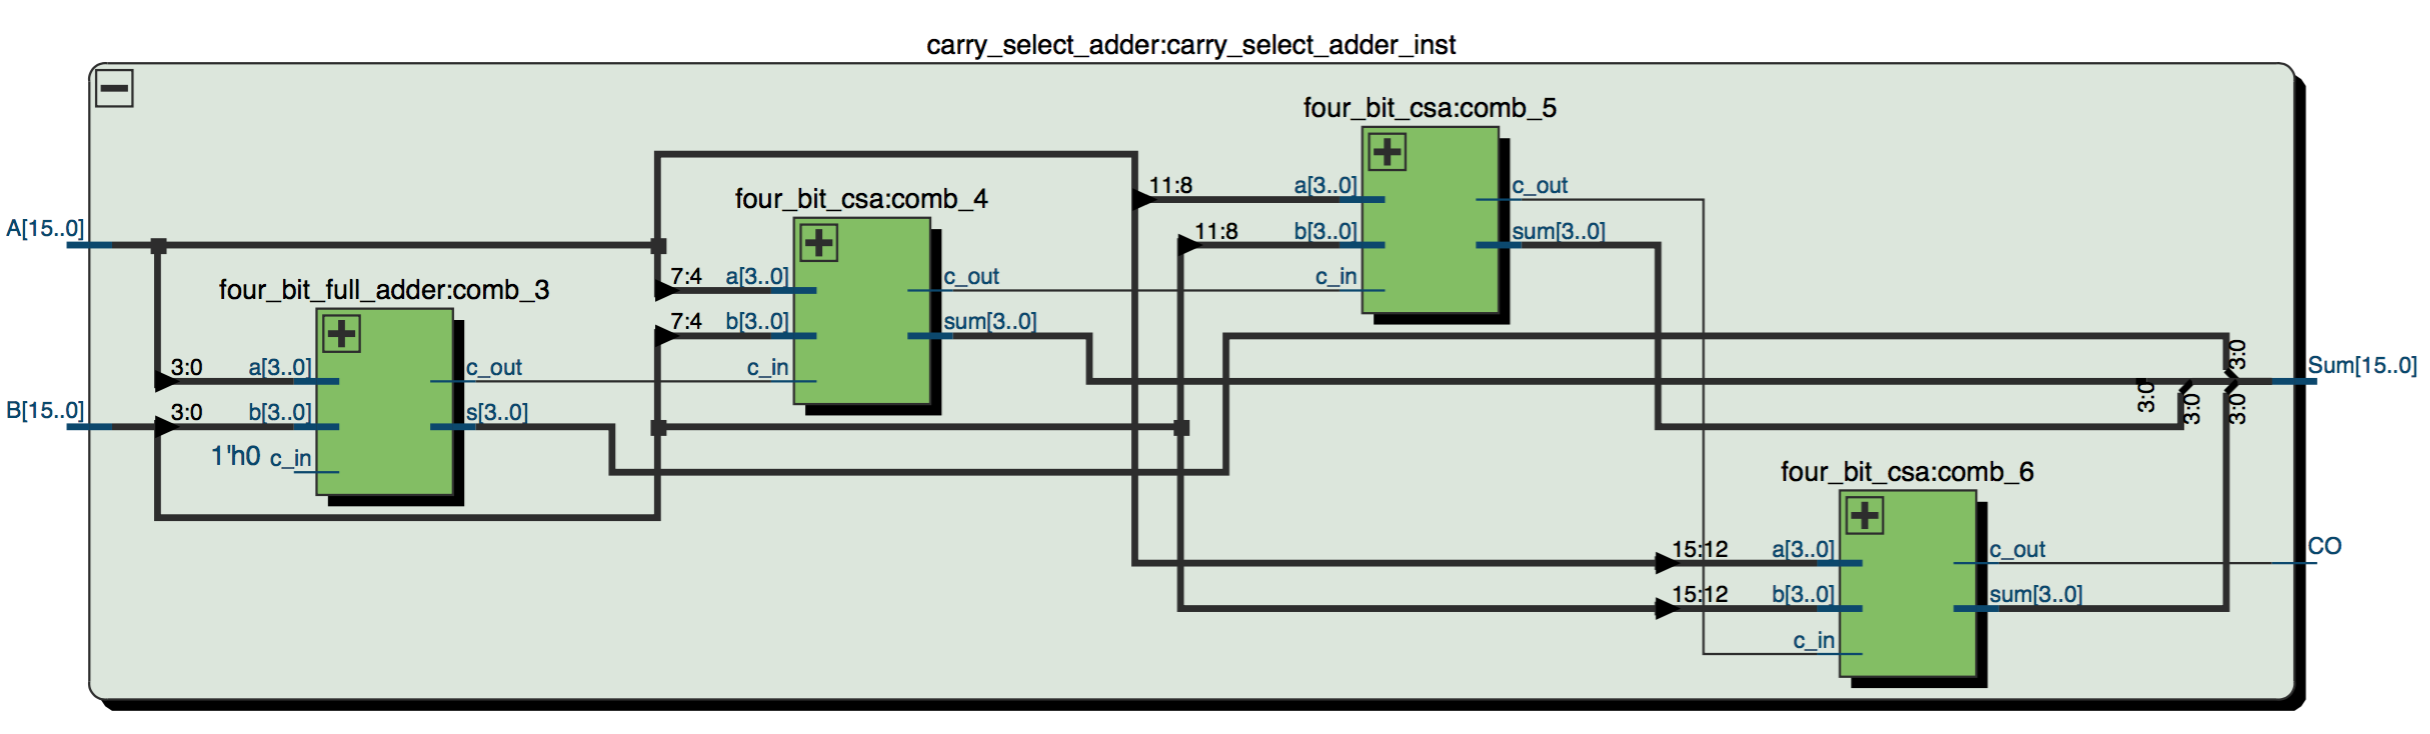
\includegraphics[scale=0.4]{carry-select-block-schematic.png}
	\caption{Carry Select (CSA) Block Schematic\label{fig:carry-select-block-schematic}}
\end{figure}

\begin{figure} [htbp]
	\centering
	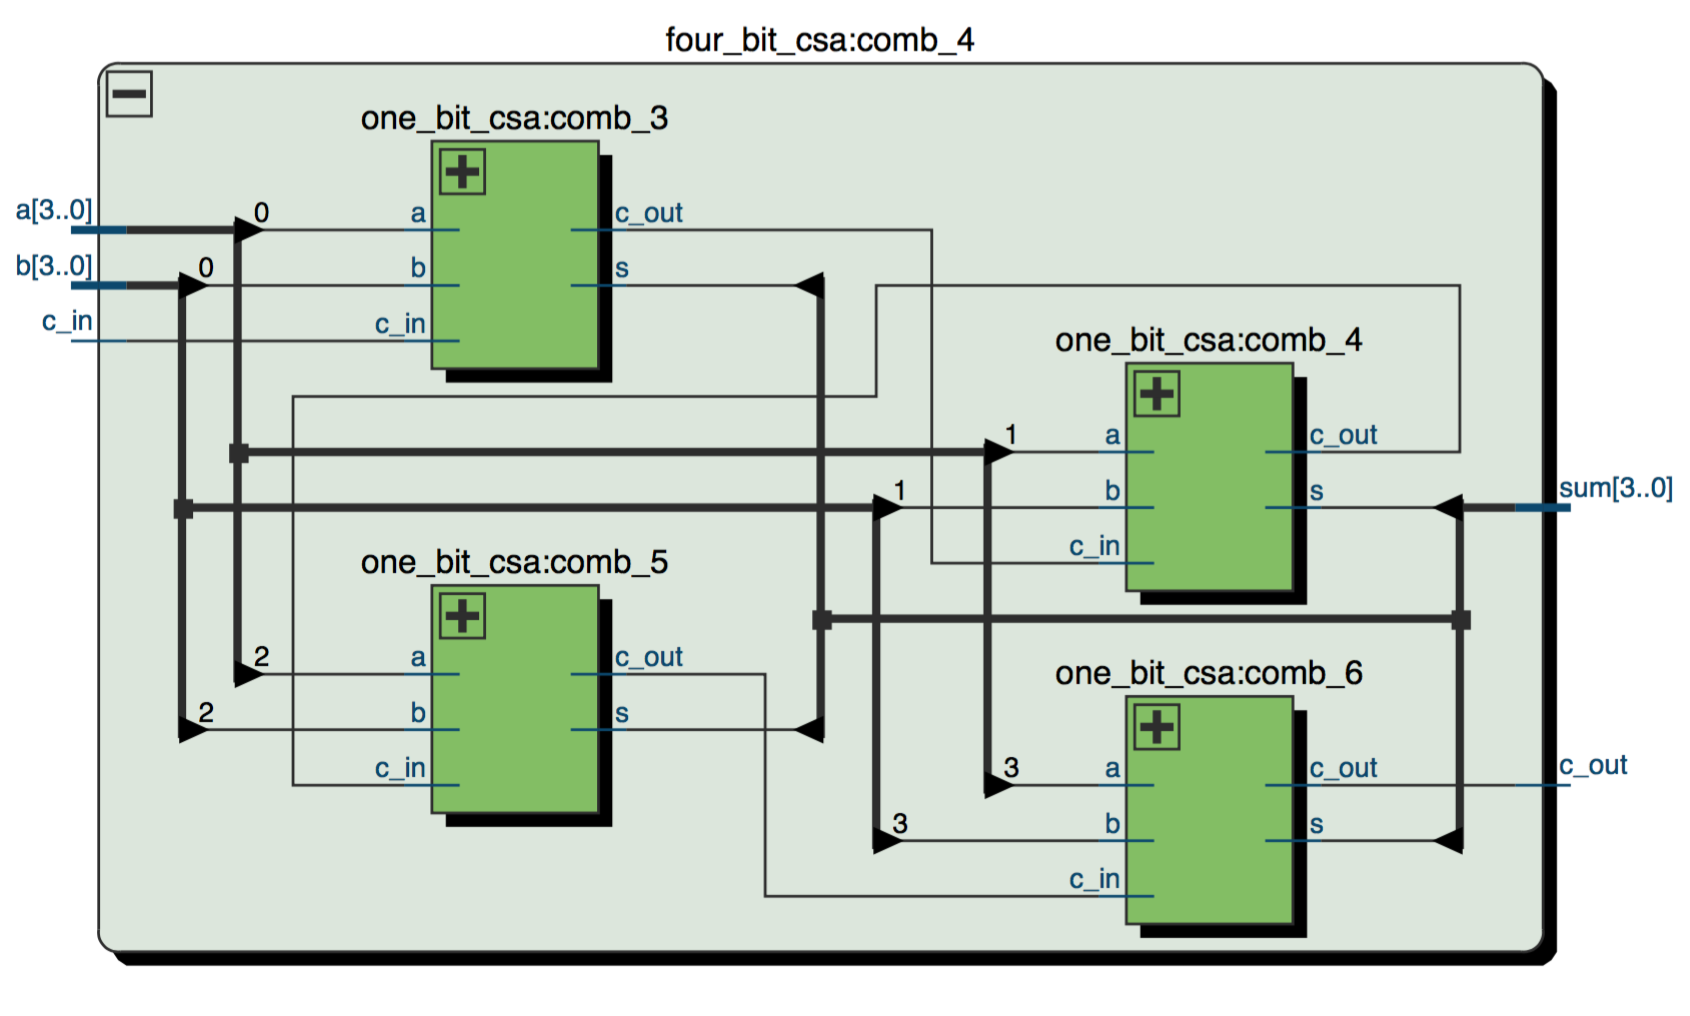
\includegraphics[scale=0.4]{four-bit-csa-block-schematic.png}
	\caption{Four-Bit CSA Block Schematic\label{fig:four-bit-csa-block-schematic}}
\end{figure}

\begin{figure} [htbp]
	\centering
	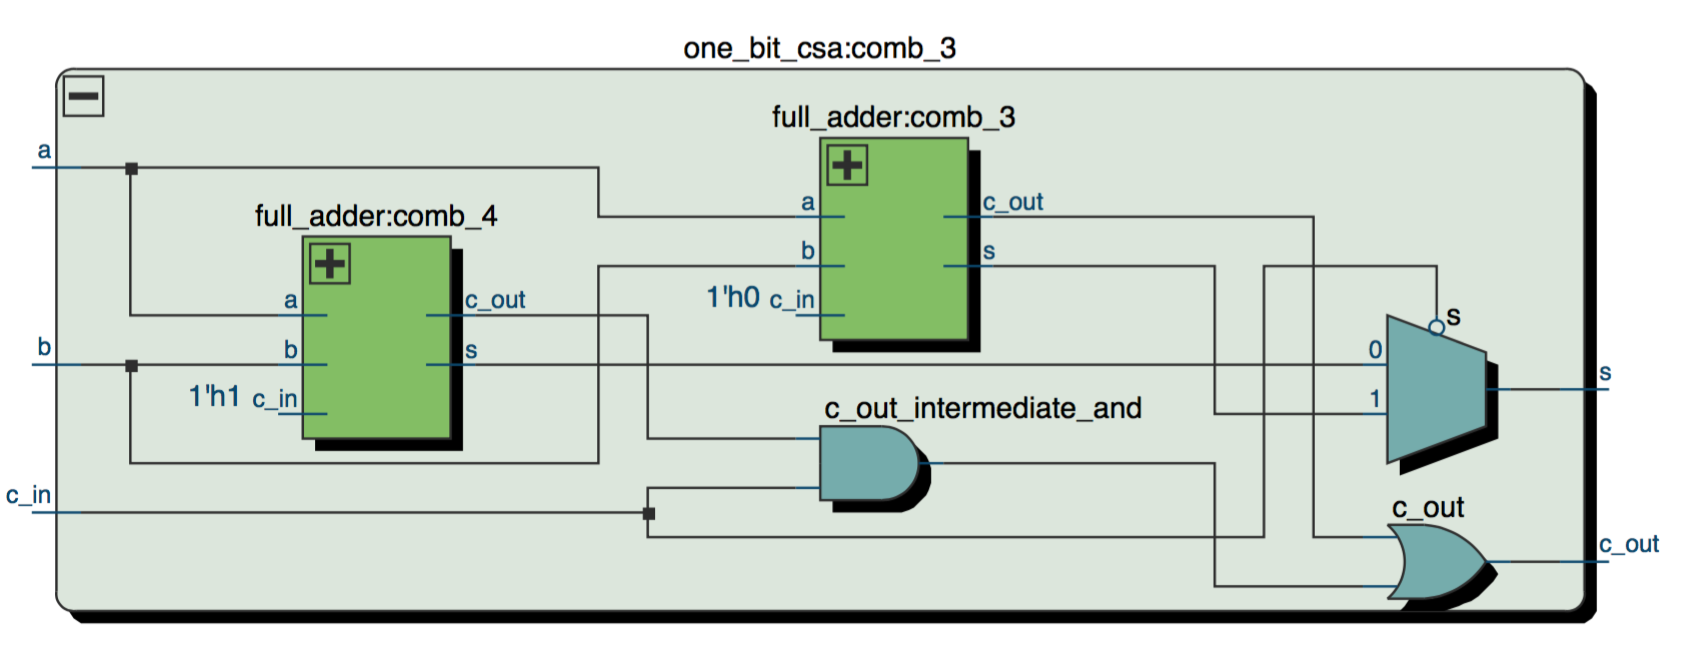
\includegraphics[scale=0.4]{one-bit-csa-block-schematic.png}
	\caption{One-Bit CSA Block Schematic\label{fig:one-bit-csa-block-schematic}}
\end{figure}




%SECTION : Bibliography
%Insert Bibliography if needed

\end{document}